% !TEX root = thesis-ex.tex
%\section{Deriving the HI JER}
%
%\subsection{Reviewing and updating the Run 1 Analysis}
%
%We will start with the starting point from the Run 1 note. Namely, we define the per-jet measure- ment errors in terms of terms that are fully correlated between EMTopo and HI collections and terms that are completely uncorrelated. For now, we assume the correlated contribution is the same for both collections.
%
%\begin{equation}
%\begin{aligned}
%\Delta\ptEM = \Delta_{c} + \Delta_{\EM} \\
%\Delta\ptHI = \Delta_{c} + \Delta_{\HI} 
%\end{aligned}
%\end{equation}
%
%Then, the jet energy resolution, defined as the standard deviation of the jet energy from the true can be written,
%\begin{equation}
%\begin{aligned}
%\REM = Var[\Delta\ptEM] = Var[\Delta_{c} +\Delta_{\EM} ] = Var[\Delta_{c}]+Var[\Delta_{\EM}] \\
%\RHI = Var[\Delta\ptHI] = Var[\Delta_{c} +\Delta_{\HI} ] = Var[\Delta_{c}]+Var[\Delta_{\HI}]
%\end{aligned}
%\end{equation}
%
%Simplifying hte notation: $Var[\Delta_{c}] = s_c^2, Var[\Delta_{\EM}] = \sEM^{2}, Var[\Delta_{\HI}] = \sHI^{2}$:
%
%\begin{equation}
%\begin{aligned}
%\REM = s_{c}^{2} + \sEM^{2} \\
%\RHI = s_{c}^{2} + \sHI^{2} \\
%\label{eq:REM_RHI}
%\end{aligned}
%\end{equation}
%
%Then defining A as the difference between the $\REM$ and $\RHI$:
%
%\begin{equation}
%\begin{aligned}
%A =  \REM - \RHI = s^{2}_{\EM} - s^{2}_{\HI}
%\end{aligned}
%\end{equation}
%
%Furthermore, we can evaluate the variance of the difference between $\Delta\pt^{\EM}$ and $\Delta\pt^{\HI}$ 
%
%\begin{equation}
%\begin{aligned}
%B_{MC} = Var[ (\Delta\ptEM -\ptHI )] =  \sEM^{2} + \sHI^2
%\end{aligned}
%\end{equation}
%
%In data them, we can get an estimate of the squared uncertainty on $B$:
%
%\begin{equation}
%\begin{aligned}
%\delta B^2 = (B_{MC} - B_{data})^2
%\end{aligned}
%\end{equation}
%
%The jet-EtMiss group has provided uncertainties on $\REM$, which we can write as $\delta^2 \REM$. Then, given these two quantities, $\delta^2 \RHI$ can be limited.
%Starting with Eq. \ref{eq:REM_RHI}:
%
%\begin{equation}
%\begin{aligned}
%\delta^2 \REM = \delta^2 s_{c}^2 + \delta^2 \sEM \\
%\delta^2 \RHI = \delta^2 s_{c}^2 + \delta^2 \sHI 
%\end{aligned}
%\end{equation}
%
%Then, given $\delta^2\REM$, $0 \leq \delta^2 s_{c}^2 \leq \delta^2 \REM$. Letting $\delta^2 s_{c}^2 = f \delta^2 \REM$, we can write $\delta^2 (1-f) \delta^2 \REM$

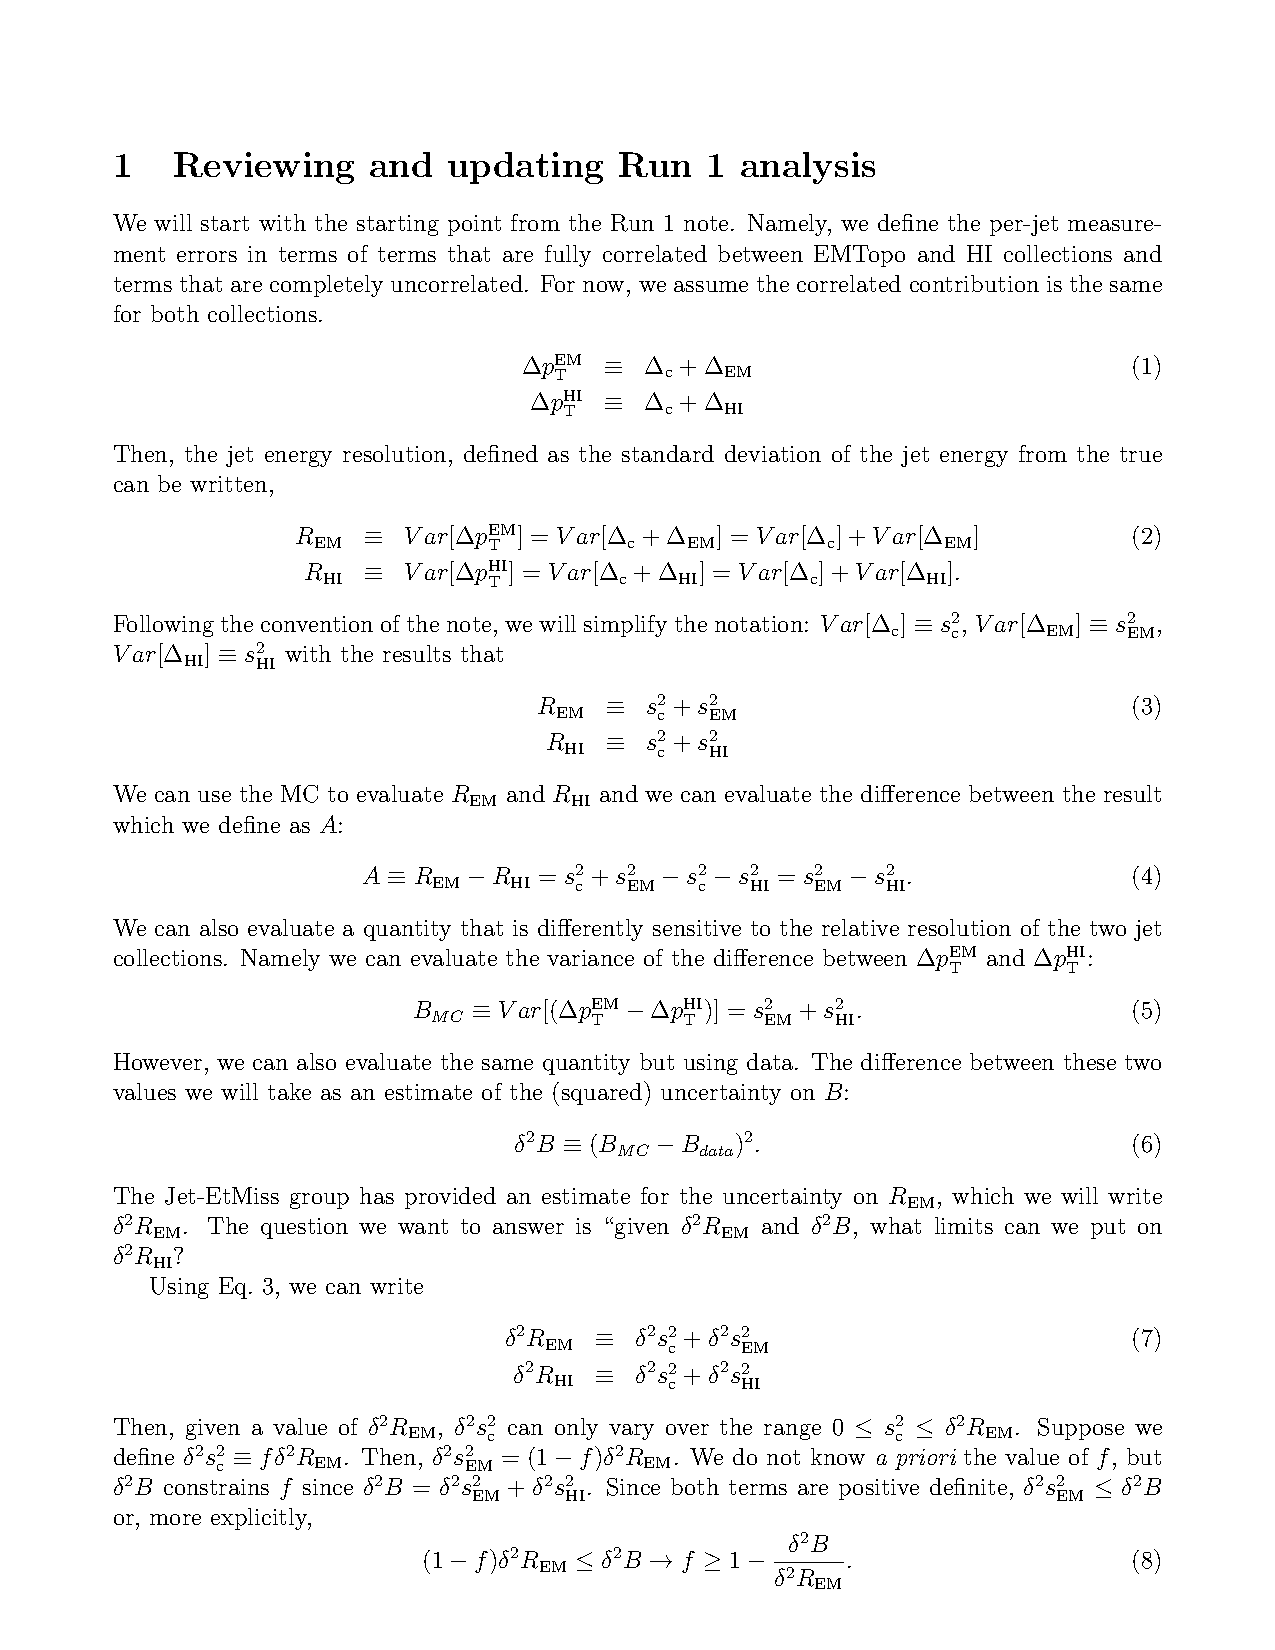
\includepdf[page={1}]{figures/appendixHIJERDerivation/JERUncertaintyNote}
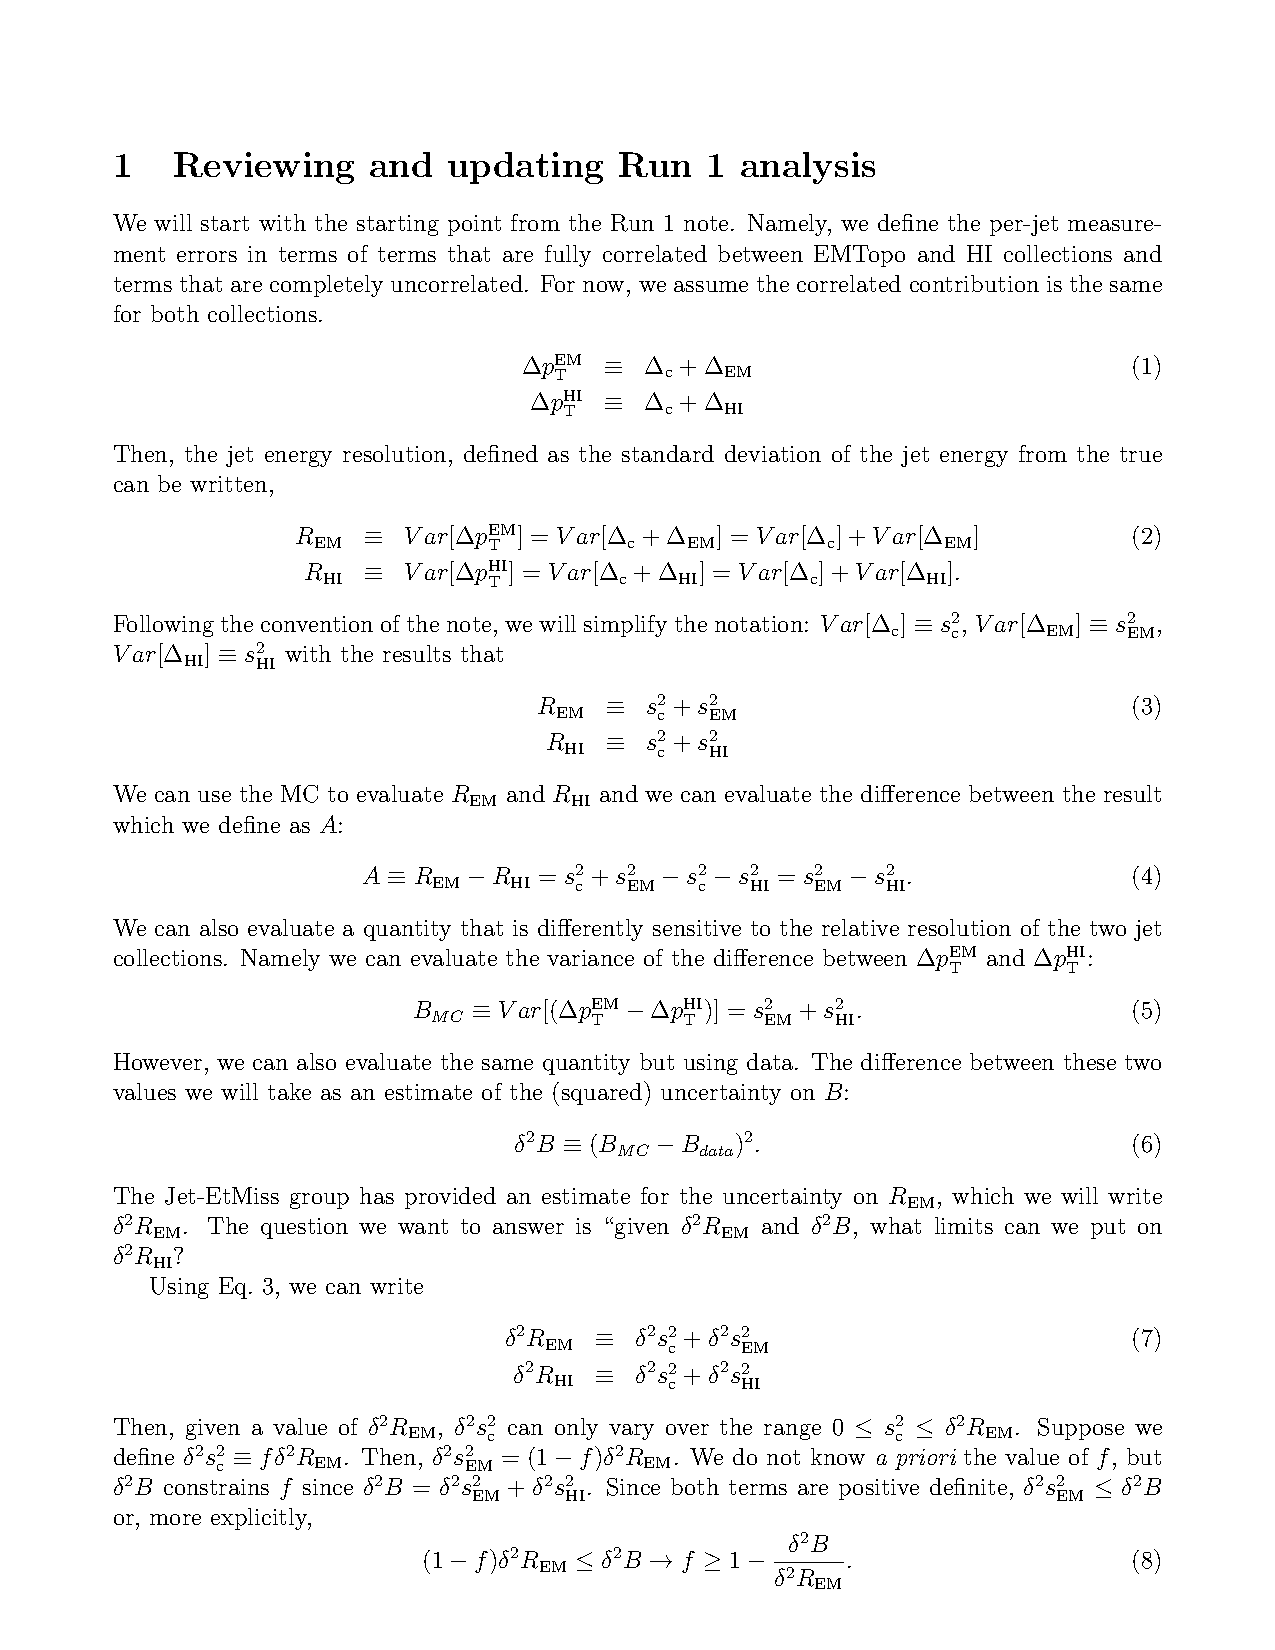
\includepdf[page={2}]{figures/appendixHIJERDerivation/JERUncertaintyNote}
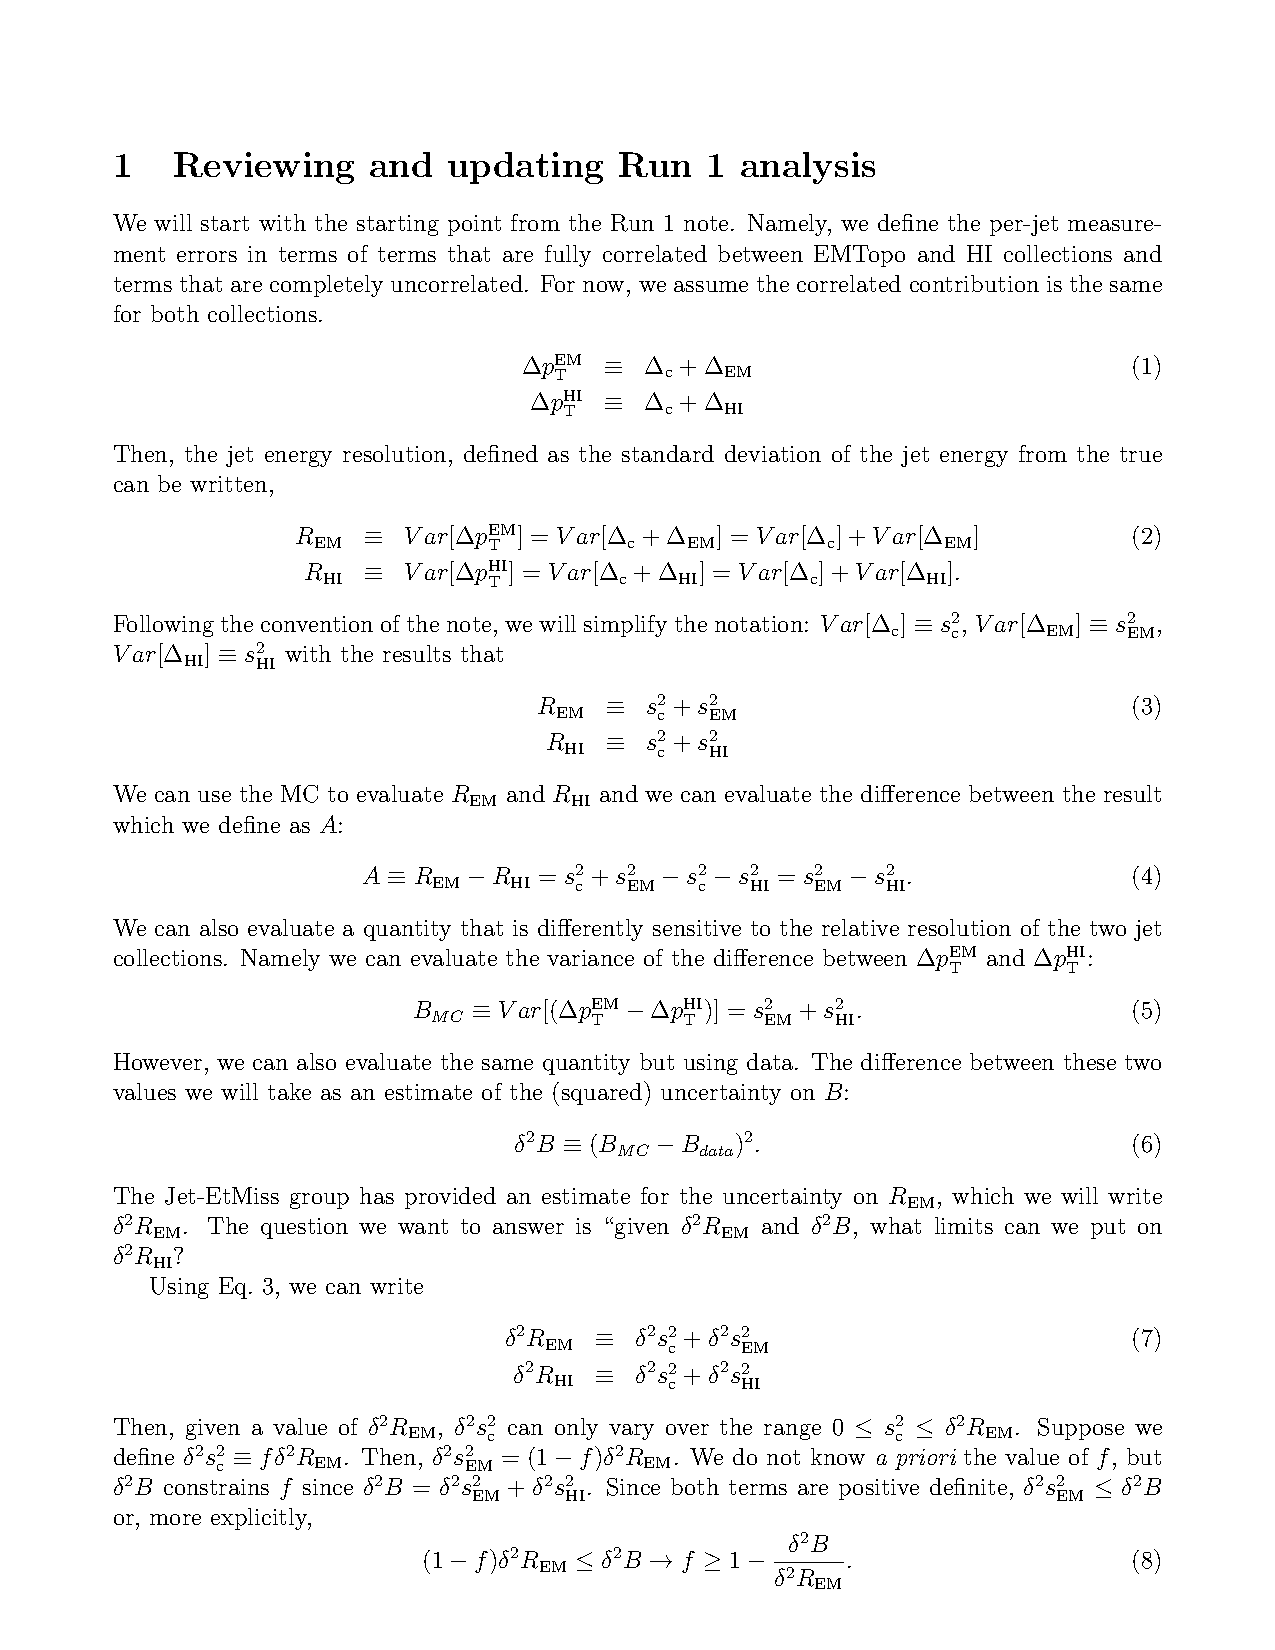
\includepdf[page={3}]{figures/appendixHIJERDerivation/JERUncertaintyNote}

%\begin{figure}
%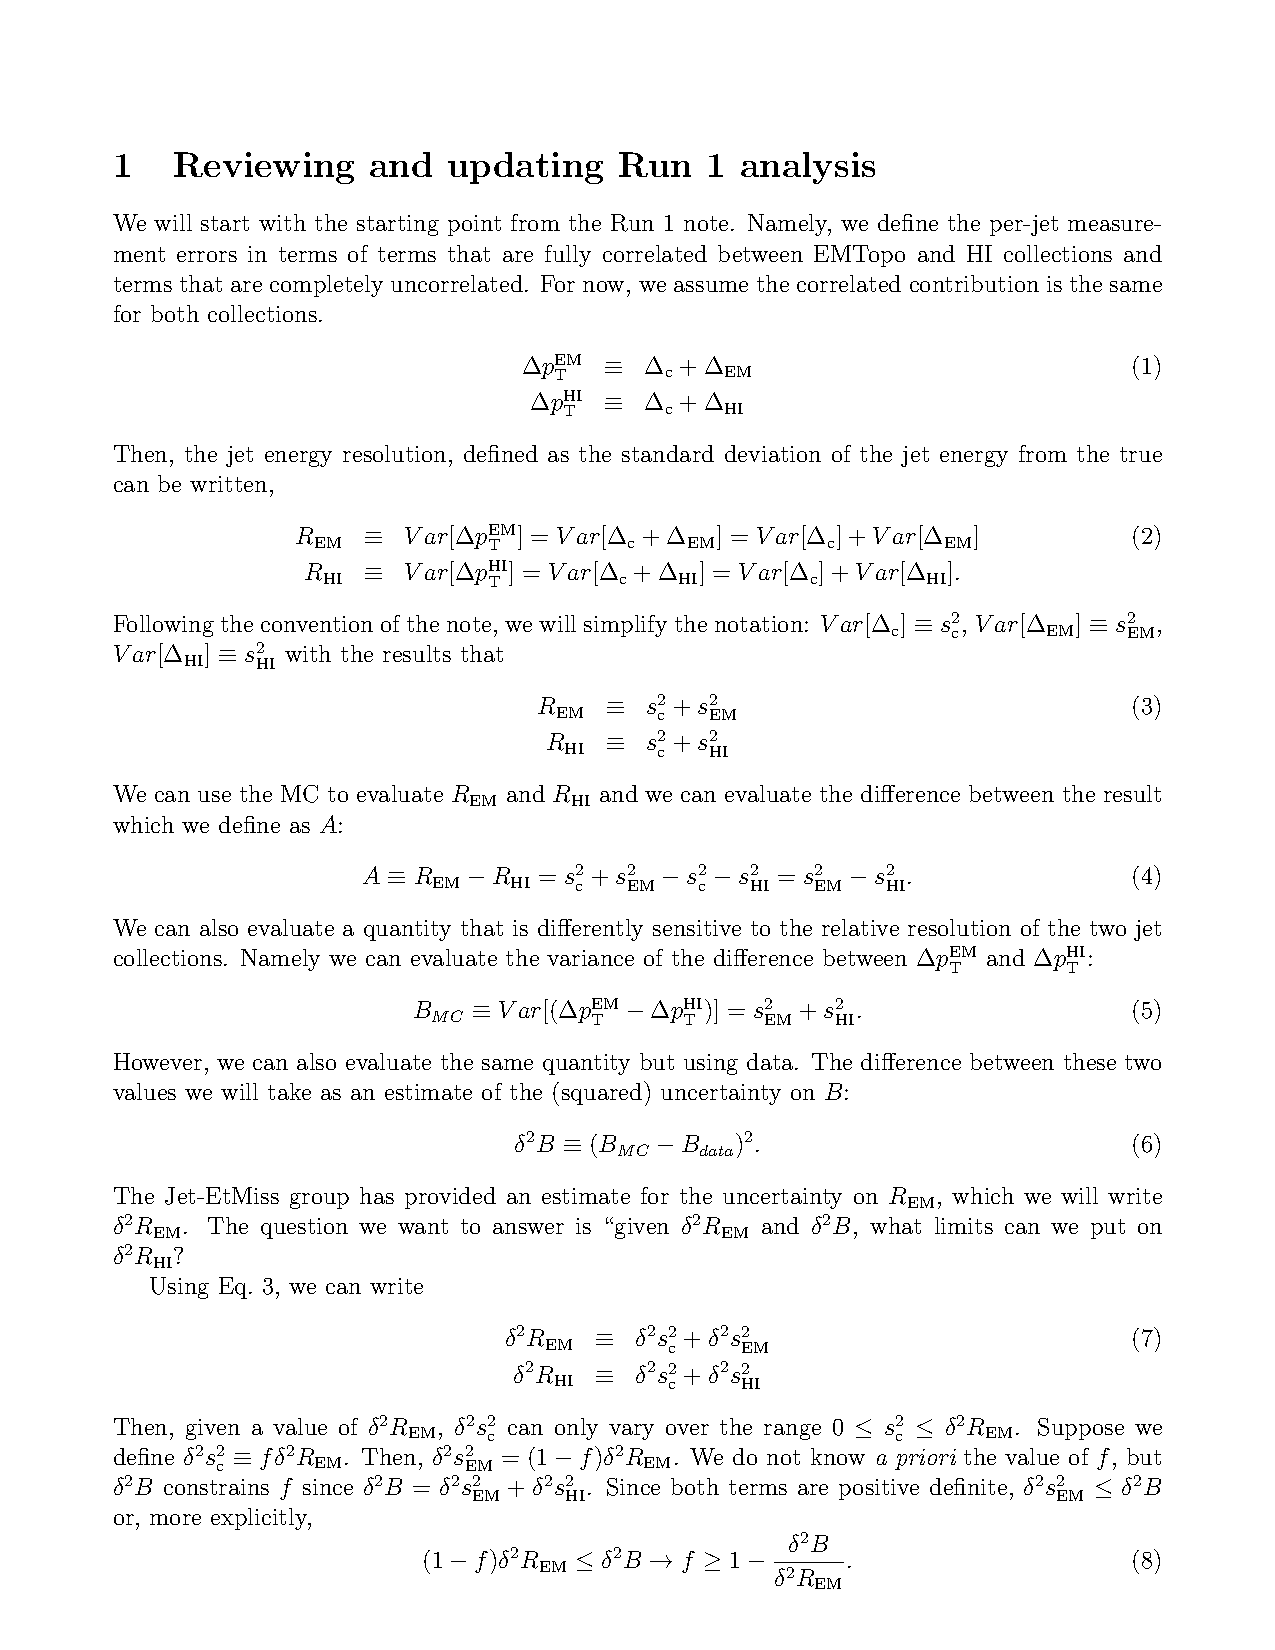
\includegraphics[page=1,width=0.7\textwidth]{figures/appendixHIJERDerivation/JERUncertaintyNote} 
%\end{figure}
%
%\begin{figure}
%\includegraphics[page=2,width=0.7\textwidth]{figures/appendixHIJERDerivation/JERUncertaintyNote} 
%\end{figure}
%
%\begin{figure}
%\includegraphics[page=3,width=0.7\textwidth]{figures/appendixHIJERDerivation/JERUncertaintyNote} 
%\end{figure}
